\begin{problem}[问题4.1]
求一加速运动的容器中盛有的液体自由面与水平面的夹角.
\begin{center}
%\includegraphics[width=0.3\textwidth]{./homework04/problem01.pdf}
\usetikzlibrary{%
    decorations.pathreplacing,%
    decorations.pathmorphing,arrows
}
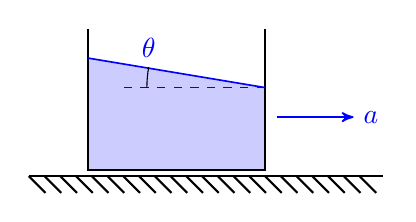
\begin{tikzpicture}[ media/.style={font={\footnotesize\sffamily}},
    interface/.style={
        postaction={draw,decorate,decoration={border,angle=-45,
                    amplitude=0.3cm,segment length=2mm}}},scale=1.5]
\draw[thick,interface](0,0)--(3,0);


\fill[blue!20](0.5,1)--(0.5,0.05)--(2,0.05)--(2,0.75);

\draw[semithick] (0.5,1.25)--(0.5,0.05)--(2,0.05)--(2,1.25);
\draw[blue, semithick] (0.5,1)--(2,0.75);
\draw[blue,dashed](2,0.75)--(0.75,0.75);
\draw (1,0.75) arc(180:170:1) node[blue,above]{$\theta$};

\draw [semithick,->,>=stealth',blue] (2.1,0.5)--(2.75,0.5) node[right]{$a$};



\end{tikzpicture}

\end{center}
\end{problem}

\begin{solution}
\textbf{解:} 均加速运动的液体相对静止, 压强除重力场外, 水平方向的惯性力也有贡献
\begin{eqnarray}
\nabla p & = & -\rho\nabla gz-\rho\nabla ax\nonumber\\
         & = & -\rho\nabla(gz+ax)\nonumber\\
         & = & -\nabla(\rho gz+\rho ax)\nonumber
\end{eqnarray}
积分得
\[
p + \rho gz+\rho ax = \mathrm{const}
\]
对于液面,压强为$p_0$, 因此对于液面上的点$(x,z)$有
\[
p_0 + \rho gz+\rho ax = \mathrm{const}\Rightarrow \frac{d(p_0 + \rho gz+\rho ax)}{dx} = 0
\]
可解得液面的斜率$dz/dx$:
\[
\frac{dz}{dx}= -\frac{a}{g}
\]
因此, 液体自由面与水平面的夹角为$\theta = \arctan (a/g)$
\end{solution} 
